\section{Results}\label{sec:results}

\subsection{RQ1: Detection quality collapses outside the random split, and AUROC hides what matters}\label{sec:rq1}

\paragraph{Data audit and leakage}
The audit (Table~\ref{tab:data}) shows that the corpora are less clean than their raw size suggests: 24.6\% of the Big-Vul rows (53\,373) are exact duplicates after normalisation, against 0.9\% for DiverseVul, and 69\,268 normalised functions occur in both corpora, i.e.\ 42.7\% of clean Big-Vul and 21.3\% of clean DiverseVul. In the cross-dataset scenarios, about 44\,000 functions of the evaluated target test part (more than a quarter of Big-Vul, and about 13\% of DiverseVul) also appear in the training data. Figure~\ref{fig:leak} and Table~\ref{tab:leak} show what this does to a naive cross-dataset evaluation: for the LR+LGBM scorer, AUPRC is $0.171$ on leak-free Big-Vul functions but $0.602$ on the leaked ones (3.5$\times$), and $0.144$ vs.\ $0.812$ (5.6$\times$) when training on Big-Vul and testing on DiverseVul. A cross-dataset result that does not remove shared functions would therefore report a performance that is between three and a half and almost six times better than what a new codebase would experience.

\begin{figure}[t]
\centering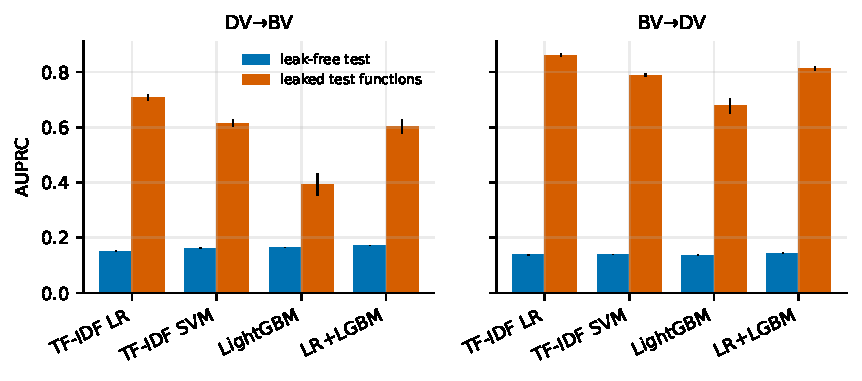
\includegraphics[width=.78\linewidth]{figs/fig_leak.pdf}
\caption{AUPRC on leak-free versus leaked cross-dataset test functions (mean $\pm$ s.d.\ over 3 seeds). The prevalence of vulnerable functions is about 5\%.}\label{fig:leak}
\end{figure}
\begin{table}[t]
\centering\footnotesize
\caption{Effect of train--test leakage in the cross-dataset setting: ``leaked'' test functions have a normalised hash that occurs in the training data.}\label{tab:leak}
\resizebox{\linewidth}{!}{\begin{tabular}{llrcccc}
\toprule
Scenario & Model & Leaked $n$ & AUPRC clean & AUPRC leaked & AUROC clean & AUROC leaked \\
\midrule
DV$\to$BV & TF-IDF LR & 44,180 & 0.151\,{\scriptsize$\pm$0.002} & 0.708\,{\scriptsize$\pm$0.010} & 0.679\,{\scriptsize$\pm$0.001} & 0.984\,{\scriptsize$\pm$0.002} \\
DV$\to$BV & LightGBM & 44,180 & 0.163\,{\scriptsize$\pm$0.000} & 0.392\,{\scriptsize$\pm$0.040} & 0.711\,{\scriptsize$\pm$0.003} & 0.877\,{\scriptsize$\pm$0.009} \\
DV$\to$BV & LR+LGBM & 44,180 & 0.171\,{\scriptsize$\pm$0.001} & 0.602\,{\scriptsize$\pm$0.026} & 0.710\,{\scriptsize$\pm$0.002} & 0.969\,{\scriptsize$\pm$0.002} \\
BV$\to$DV & TF-IDF LR & 44,120 & 0.137\,{\scriptsize$\pm$0.001} & 0.862\,{\scriptsize$\pm$0.005} & 0.711\,{\scriptsize$\pm$0.001} & 0.951\,{\scriptsize$\pm$0.003} \\
BV$\to$DV & LightGBM & 44,120 & 0.136\,{\scriptsize$\pm$0.002} & 0.679\,{\scriptsize$\pm$0.027} & 0.709\,{\scriptsize$\pm$0.006} & 0.909\,{\scriptsize$\pm$0.007} \\
BV$\to$DV & LR+LGBM & 44,120 & 0.144\,{\scriptsize$\pm$0.002} & 0.812\,{\scriptsize$\pm$0.007} & 0.721\,{\scriptsize$\pm$0.003} & 0.948\,{\scriptsize$\pm$0.002} \\
\bottomrule
\end{tabular}}
\end{table}


\paragraph{Performance under shift}
Table~\ref{tab:detect} and Figure~\ref{fig:detection} give the detection results. On random splits the LR+LGBM scorer reaches AUPRC $0.248$ (DiverseVul) and $0.407$ (Big-Vul); the percentages below are drops of this scorer, with AUROC $0.836$ and $0.869$. When whole projects are held out, AUPRC falls to $0.141$ (\,$-43\%$) and $0.151$ (\,$-63\%$); the temporal split on Big-Vul yields $0.113$ (\,$-72\%$), and the leak-free cross-dataset settings give $0.171$ and $0.144$. These values are only two to three times the prevalence ($\approx5\%$), and MCC drops to $0.12$--$0.17$ for the best model (Table~\ref{tab:detect}, panel C), against $0.29$ and $0.39$ on random splits. The ID-calibration AUPRC (what a practitioner would see on a hold-out of the training distribution) is $0.24$--$0.43$ in every scenario, so the optimism of in-distribution validation reaches $1.5$--$3.8\times$ for project, temporal and cross-dataset deployment ($0.264$ vs.\ $0.141$ for DiverseVul project, $0.425$ vs.\ $0.113$ for Big-Vul temporal).
The Friedman test over the 21 scenario--seed blocks rejects equal AUPRC for the four scorers ($\chi^2=21.9$, $p<10^{-4}$); the LR+LGBM scorer has the best mean rank ($1.48$), and beats TF-IDF LR ($p=0.011$, Cliff's $\delta=0.18$) and LightGBM ($p<10^{-5}$, $\delta=0.14$), while the difference to the SVM is borderline ($p=0.055$, $\delta=0.14$). Differences between scorers are small relative to the drop caused by the evaluation setting. We therefore use LR+LGBM as the scorer in the triage experiments unless stated otherwise.

\begin{figure}[t]
\centering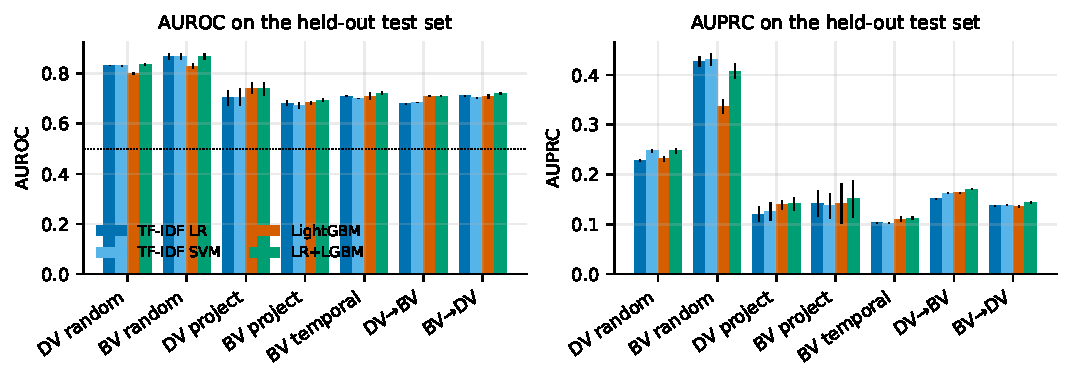
\includegraphics[width=\linewidth]{figs/fig_detection.pdf}
\caption{Detection performance of the four scorers across the seven scenarios (mean $\pm$ s.d.\ over 3 seeds).}\label{fig:detection}
\end{figure}
\begin{table}[t]
\centering\small
\caption{Detection performance on the held-out test sets (mean $\pm$ s.d.\ over 3 seeds; best per row in bold). MCC uses the F1-optimal threshold chosen on ID calibration data.}\label{tab:detect}
\begin{tabular}{lcccc}
\toprule
Scenario & TF-IDF LR & TF-IDF SVM & LightGBM & LR+LGBM \\
\midrule
\multicolumn{5}{l}{\emph{Panel A: AUPRC}} \\
DV random & 0.229\,{\scriptsize$\pm$0.002} & \textbf{0.248\,{\scriptsize$\pm$0.003}} & 0.231\,{\scriptsize$\pm$0.004} & 0.248\,{\scriptsize$\pm$0.005} \\
BV random & 0.427\,{\scriptsize$\pm$0.010} & \textbf{0.432\,{\scriptsize$\pm$0.012}} & 0.337\,{\scriptsize$\pm$0.013} & 0.407\,{\scriptsize$\pm$0.015} \\
DV project & 0.120\,{\scriptsize$\pm$0.015} & 0.126\,{\scriptsize$\pm$0.018} & 0.139\,{\scriptsize$\pm$0.009} & \textbf{0.141\,{\scriptsize$\pm$0.013}} \\
BV project & 0.142\,{\scriptsize$\pm$0.027} & 0.137\,{\scriptsize$\pm$0.025} & 0.143\,{\scriptsize$\pm$0.040} & \textbf{0.151\,{\scriptsize$\pm$0.037}} \\
BV temporal & 0.103\,{\scriptsize$\pm$0.001} & 0.102\,{\scriptsize$\pm$0.000} & 0.110\,{\scriptsize$\pm$0.005} & \textbf{0.113\,{\scriptsize$\pm$0.003}} \\
DV$\to$BV & 0.151\,{\scriptsize$\pm$0.002} & 0.162\,{\scriptsize$\pm$0.001} & 0.163\,{\scriptsize$\pm$0.000} & \textbf{0.171\,{\scriptsize$\pm$0.001}} \\
BV$\to$DV & 0.137\,{\scriptsize$\pm$0.001} & 0.139\,{\scriptsize$\pm$0.001} & 0.136\,{\scriptsize$\pm$0.002} & \textbf{0.144\,{\scriptsize$\pm$0.002}} \\
\midrule
\multicolumn{5}{l}{\emph{Panel B: AUROC}} \\
DV random & 0.832\,{\scriptsize$\pm$0.001} & 0.832\,{\scriptsize$\pm$0.002} & 0.800\,{\scriptsize$\pm$0.002} & \textbf{0.836\,{\scriptsize$\pm$0.002}} \\
BV random & \textbf{0.869\,{\scriptsize$\pm$0.013}} & 0.867\,{\scriptsize$\pm$0.012} & 0.830\,{\scriptsize$\pm$0.010} & 0.869\,{\scriptsize$\pm$0.012} \\
DV project & 0.704\,{\scriptsize$\pm$0.030} & 0.706\,{\scriptsize$\pm$0.033} & \textbf{0.742\,{\scriptsize$\pm$0.022}} & 0.740\,{\scriptsize$\pm$0.026} \\
BV project & 0.683\,{\scriptsize$\pm$0.012} & 0.674\,{\scriptsize$\pm$0.012} & 0.684\,{\scriptsize$\pm$0.006} & \textbf{0.694\,{\scriptsize$\pm$0.005}} \\
BV temporal & 0.710\,{\scriptsize$\pm$0.002} & 0.701\,{\scriptsize$\pm$0.001} & 0.710\,{\scriptsize$\pm$0.013} & \textbf{0.722\,{\scriptsize$\pm$0.006}} \\
DV$\to$BV & 0.679\,{\scriptsize$\pm$0.001} & 0.685\,{\scriptsize$\pm$0.001} & \textbf{0.711\,{\scriptsize$\pm$0.003}} & 0.710\,{\scriptsize$\pm$0.002} \\
BV$\to$DV & 0.711\,{\scriptsize$\pm$0.001} & 0.704\,{\scriptsize$\pm$0.002} & 0.709\,{\scriptsize$\pm$0.006} & \textbf{0.721\,{\scriptsize$\pm$0.003}} \\
\midrule
\multicolumn{5}{l}{\emph{Panel C: MCC}} \\
DV random & \textbf{0.292\,{\scriptsize$\pm$0.004}} & 0.291\,{\scriptsize$\pm$0.006} & 0.257\,{\scriptsize$\pm$0.002} & 0.288\,{\scriptsize$\pm$0.006} \\
BV random & \textbf{0.415\,{\scriptsize$\pm$0.013}} & 0.413\,{\scriptsize$\pm$0.018} & 0.319\,{\scriptsize$\pm$0.011} & 0.387\,{\scriptsize$\pm$0.014} \\
DV project & 0.120\,{\scriptsize$\pm$0.025} & 0.134\,{\scriptsize$\pm$0.024} & 0.163\,{\scriptsize$\pm$0.030} & \textbf{0.165\,{\scriptsize$\pm$0.030}} \\
BV project & 0.112\,{\scriptsize$\pm$0.032} & 0.109\,{\scriptsize$\pm$0.036} & 0.125\,{\scriptsize$\pm$0.052} & \textbf{0.133\,{\scriptsize$\pm$0.057}} \\
BV temporal & 0.071\,{\scriptsize$\pm$0.011} & 0.073\,{\scriptsize$\pm$0.008} & 0.119\,{\scriptsize$\pm$0.007} & \textbf{0.121\,{\scriptsize$\pm$0.016}} \\
DV$\to$BV & 0.150\,{\scriptsize$\pm$0.007} & 0.161\,{\scriptsize$\pm$0.004} & 0.158\,{\scriptsize$\pm$0.005} & \textbf{0.166\,{\scriptsize$\pm$0.002}} \\
BV$\to$DV & 0.138\,{\scriptsize$\pm$0.002} & 0.146\,{\scriptsize$\pm$0.007} & 0.140\,{\scriptsize$\pm$0.006} & \textbf{0.149\,{\scriptsize$\pm$0.007}} \\
\bottomrule
\end{tabular}
\end{table}


\paragraph{AUROC is a poor proxy for operational value}
By Lemma~\ref{lem:auc}, AUROC averages the clearable fraction of benign functions over all miss budgets. A team that wants at most $5\%$ of vulnerabilities cleared by the tool uses only the left tail. Across the 84 scorer--scenario--seed combinations, the Spearman correlation between AUROC and the share of functions that can be cleared at $\alpha=5\%$ is only $\rho=0.38$. Within a scenario, scorers whose mean AUROC differs by $0.02$--$0.04$ differ by $0.04$--$0.13$ in clearable share (e.g.\ DiverseVul random: AUROC range $0.036$, SAR range $0.114$). Model selection for triage must therefore use the operating point of interest, not a global ranking metric.

\paragraph{A formatting shortcut in the Big-Vul release} While preparing the pre-trained-model experiment (Section~\ref{sec:rq6}) we found that the raw text of the Hugging Face release of Big-Vul carries a strong formatting signal: a classifier that sees only 15 formatting statistics (indentation, trailing whitespace, comment markers, line lengths; Table~\ref{tab:format}) reaches AUROC $0.919$ on a random split, higher than every semantic model in this paper (the raw-text CodeBERT ensemble of Section~\ref{sec:rq6}, which also sees the formatting, comes close at $0.893$), and whitespace structure alone (tabs, leading and trailing whitespace, indentation, brace placement) reaches $0.892$ against $0.687$ for size alone (Table~\ref{tab:formatabl}). The signal is present in PrimeVul as well (whitespace structure alone $0.841$) but not in DiverseVul, where size dominates ($0.719$ for size alone, $0.682$ for whitespace). All detectors in Sections~\ref{sec:rq1}--\ref{sec:rq5} operate on comment-stripped, whitespace-insensitive tokens and code metrics, and removing the only size-sensitive metrics (characters, lines, tokens) changes the AUROC of the LightGBM scorer by at most $0.006$ ($0.820\to0.818$ on Big-Vul, $0.801\to0.802$ on DiverseVul, $0.820\to0.814$ on PrimeVul), so the main results are not driven by it (the same holds on PrimeVul, Section~\ref{sec:rq8}); but results obtained by models that read raw Big-Vul text should be interpreted with this in mind.

\subsection{RQ2: Calibration is acceptable in-distribution and degrades under shift}\label{sec:rq2}
Table~\ref{tab:calib} reports ECE. Raw probabilities are mildly miscalibrated even on random splits (LR: $0.015$--$0.032$; LightGBM: $0.0075$--$0.018$), largely because training keeps at most 150\,000 benign functions. Platt scaling and isotonic regression fitted on ID calibration data reduce ECE to $0.004$--$0.015$ on random splits, but under shift the residual error is much larger: $0.014$--$0.030$ (LR and LightGBM, Platt scaling and isotonic regression) for the project, temporal and cross-dataset settings, i.e.\ roughly $30$--$60\%$ of the 5\% base rate, and the two methods perform alike. The one exception is LightGBM trained on DiverseVul and tested on Big-Vul, where raw probabilities ($0.008$) beat recalibrated ones ($0.018$). Importantly, because the clearance rule depends only on the ranking of scores, post-hoc calibration changes \emph{no} triage decision; calibration matters for reporting probabilities and for cost-based decisions, not for the miss-rate guarantee.
\begin{table}[t]
\centering\footnotesize
\caption{Expected calibration error (ECE, lower is better) on the test sets; Platt scaling and isotonic regression are fitted on ID calibration data. Mean over 3 seeds.}\label{tab:calib}
\resizebox{\linewidth}{!}{\begin{tabular}{lcccccc}
\toprule
Scenario & LR raw & LR Platt & LR isotonic & LGBM raw & LGBM Platt & LGBM isotonic \\
\midrule
DV random & 0.032 & 0.015 & 0.006 & 0.018 & 0.006 & 0.004 \\
BV random & 0.015 & 0.004 & 0.004 & 0.008 & 0.005 & 0.004 \\
DV project & 0.026 & 0.010 & 0.017 & 0.009 & 0.005 & 0.008 \\
BV project & 0.037 & 0.022 & 0.023 & 0.025 & 0.022 & 0.023 \\
BV temporal & 0.022 & 0.015 & 0.016 & 0.016 & 0.016 & 0.016 \\
DV$\to$BV & 0.031 & 0.020 & 0.021 & 0.008 & 0.018 & 0.018 \\
BV$\to$DV & 0.035 & 0.023 & 0.026 & 0.022 & 0.022 & 0.023 \\
\bottomrule
\end{tabular}}
\end{table}


\subsection{RQ3: The miss-rate guarantee holds under exchangeability and fails under shift}\label{sec:rq3}

\paragraph{Validity on exchangeable splits}
Figure~\ref{fig:validity} (left) and Table~\ref{tab:alpha} show that on random splits the realised miss rate matches the nominal budget: at $\alpha=10\%$ it is $10.1\%$ (DiverseVul) and $8.6\%$ (Big-Vul); over all budgets and seeds the excess over $\alpha$ is $-0.4$ percentage points on average (one-sided Wilcoxon $p=0.80$ for ``exceeds''), and the realised-to-nominal ratio is $0.96$. This confirms Proposition~\ref{prop:valid} on real detector scores. At this budget the rule clears $54$--$55\%$ of all functions (SAR; Figure~\ref{fig:sar}), i.e.\ it reduces the number of functions that must be reviewed per 1\,000 from $1000$ to about $450$.

\begin{figure}[t]
\centering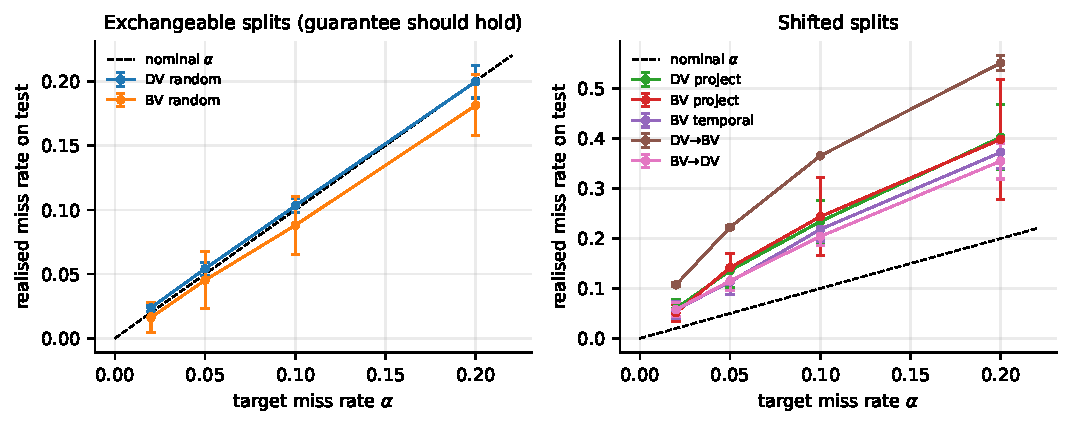
\includegraphics[width=\linewidth]{figs/fig_validity.pdf}
\caption{Realised versus nominal miss rate for source-calibrated conformal clearance (LR+LGBM scorer; mean $\pm$ s.d.\ over seeds). The dashed line is the target.}\label{fig:validity}
\end{figure}

\paragraph{Failure under shift}
In every shifted scenario the guarantee is violated (Figure~\ref{fig:validity}, right). At $\alpha=10\%$ the realised miss rate is $24.0\%$ (Big-Vul project), $23.6\%$ (DiverseVul project), $21.7\%$ (Big-Vul temporal), $20.3\%$ (Big-Vul$\to$DiverseVul) and $37.0\%$ (DiverseVul$\to$Big-Vul), on average $2.7\times$ the budget (excess $+12.8$ points, $p<10^{-11}$). At $\alpha=2\%$ the miss rates are $5.0$--$10.7\%$. The severity of the project-level violation depends on which projects are held out: for Big-Vul project the realised miss rate at $\alpha=10\%$ is $16.9$, $32.0$ and $23.0\%$ in the three partitions (and $9.4$, $17.7$ and $3.0\%$ in the three partitions of the subsample used in Section~\ref{sec:rq6}, for the normalised CodeBERT ensemble, where it can even fall below the nominal level), whereas the temporal and cross-dataset violations are stable across seeds ($20.1$--$24.2\%$, $18.3$--$22.0\%$, and $36.7$--$37.2\%$). Project shift is thus a high-variance threat, temporal and dataset shift a consistent one. Meanwhile the SAR reported for the invalid rule is deceptively high ($47.6$--$66.1\%$, Table~\ref{tab:guar}), so a team calibrating on a convenient hold-out would believe the tool is both safe and efficient.
Proposition~\ref{prop:shift} bounds the excess by the KS distance between the scores of calibration and test positives; Figure~\ref{fig:ks} shows that all $336$ (scenario, seed, scorer, $\alpha$) points lie below the bound. The excess is strongly related to the shift ($\rho=0.74$). The bound is conservative in typical cases (the KS distance is a median $3.1\times$ the excess, inter-quartile range $1.9$--$6.2$) but nearly tight in the worst one (excess up to $95\%$ of the KS distance), so it is a safe diagnostic, usable only if some labelled target positives exist.

\begin{figure}[t]
\centering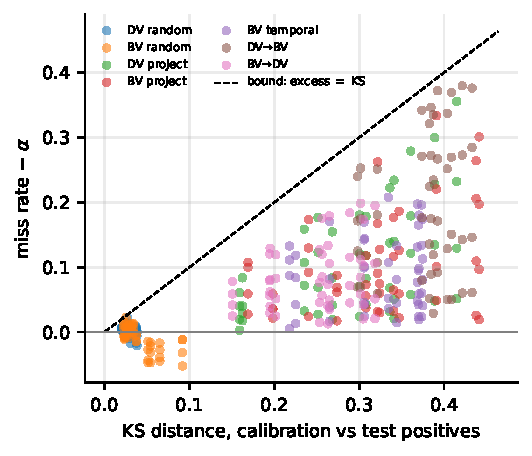
\includegraphics[width=.62\linewidth]{figs/fig_ks_bound.pdf}
\caption{Excess miss rate over the nominal budget versus the KS distance between calibration and test positive scores, for all scorers, budgets and seeds (336 points). All points lie below the diagonal bound of Proposition~\ref{prop:shift}.}\label{fig:ks}
\end{figure}
\begin{table}[t]
\centering\small
\caption{Realised miss rate (\%, mean $\pm$ s.d.\ over seeds) of the conformal clearance rule calibrated on source-distribution (ID) data, for four nominal budgets $\alpha$ (LR+LGBM scorer).}\label{tab:alpha}
\begin{tabular}{lcccc}
\toprule
Scenario & $\alpha{=}2\%$ & $\alpha{=}5\%$ & $\alpha{=}10\%$ & $\alpha{=}20\%$ \\
\midrule
DV random & 2.4{\scriptsize$\pm$0.2} & 5.5{\scriptsize$\pm$0.5} & 10.1{\scriptsize$\pm$0.6} & 19.8{\scriptsize$\pm$1.7} \\
BV random & 1.5{\scriptsize$\pm$1.2} & 4.6{\scriptsize$\pm$2.5} & 8.6{\scriptsize$\pm$2.3} & 18.2{\scriptsize$\pm$2.3} \\
DV project & 5.9{\scriptsize$\pm$1.6} & 13.8{\scriptsize$\pm$3.0} & 23.6{\scriptsize$\pm$3.8} & 40.5{\scriptsize$\pm$6.5} \\
BV project & 5.0{\scriptsize$\pm$1.6} & 13.5{\scriptsize$\pm$2.1} & 24.0{\scriptsize$\pm$7.6} & 39.8{\scriptsize$\pm$12.5} \\
BV temporal & 5.6{\scriptsize$\pm$1.1} & 11.5{\scriptsize$\pm$3.0} & 21.7{\scriptsize$\pm$2.2} & 37.4{\scriptsize$\pm$3.2} \\
DV$\to$BV & 10.7{\scriptsize$\pm$0.6} & 22.4{\scriptsize$\pm$0.3} & 37.0{\scriptsize$\pm$0.3} & 55.3{\scriptsize$\pm$1.6} \\
BV$\to$DV & 5.9{\scriptsize$\pm$1.6} & 11.2{\scriptsize$\pm$2.0} & 20.3{\scriptsize$\pm$1.9} & 35.8{\scriptsize$\pm$3.4} \\
\bottomrule
\end{tabular}
\end{table}


\paragraph{Remedies}
Table~\ref{tab:guar} and Figure~\ref{fig:recal} compare the remedies at $\alpha=10\%$.
\emph{Covariate-shift weighting} helps in two scenarios (DiverseVul project: $23.6\to15.1\%$; DiverseVul$\to$Big-Vul: $37.0\to14.9\%$) but not in the other three (Big-Vul project $24.0\to18.6\%$, Big-Vul temporal $21.7\to22.6\%$, Big-Vul$\to$DiverseVul $20.3\to19.5\%$); on these two corpora it never restores the budget. The estimated weights are extremely skewed: the cap of 20 is reached for $22\%$ of the Big-Vul test functions in DiverseVul$\to$Big-Vul and for $15\%$ in Big-Vul project (median test weight $5.5$ and $5.4$ against calibration weights around $0.2$--$0.3$), so a few calibration positives carry most of the weight and the effective calibration size is small; together with a probably violated covariate-shift assumption for code, this explains why weighting is not a reliable repair.
\emph{Recalibration on labelled target positives} restores the budget: with $k=100$ the realised miss rate is $9.2$--$13.0\%$ across the five shifted scenarios (four of the five scenarios are within $10\%\pm0.8$ points; Big-Vul project is high at $13.0\%$), with a SAR of $26.7$--$31.8\%$; $k=50$ already gives $9.2$--$12.1\%$, and $k=25$ is conservative ($7.3$--$9.6\%$) because the finite-sample correction clears only $\lfloor0.1\cdot26\rfloor=2$ order statistics. The empirical curves fall inside the Beta band predicted by Corollary~\ref{cor:beta}, except for Big-Vul project at $k\ge200$, which stays slightly above it ($13.4\%$ against an upper band edge of about $12.6\%$), possibly because the projects of the target pool and of the test set differ. Because the guarantee is in expectation, the frequency with which a single calibration draw exceeds $\alpha+2$ points is $16$--$68\%$ at $k=100$; the PAC variant (Proposition~\ref{prop:pac}) cuts this to $\le7\%$ in all scenarios (mostly $\le2.3\%$), at the price of a lower SAR ($15.9$--$22.4\%$). The valid operating points under shift thus clear about $27$--$32\%$ of functions (non-PAC) or $16$--$22$\% (PAC), roughly half and a third of the $54$--$55\%$ available on random splits. Importantly, the PAC rule calibrated on \emph{source} data remains invalid under shift ($94$--$100\%$ violations), which confirms that the issue is exchangeability and not the choice of the quantile.

\begin{figure}[t]
\centering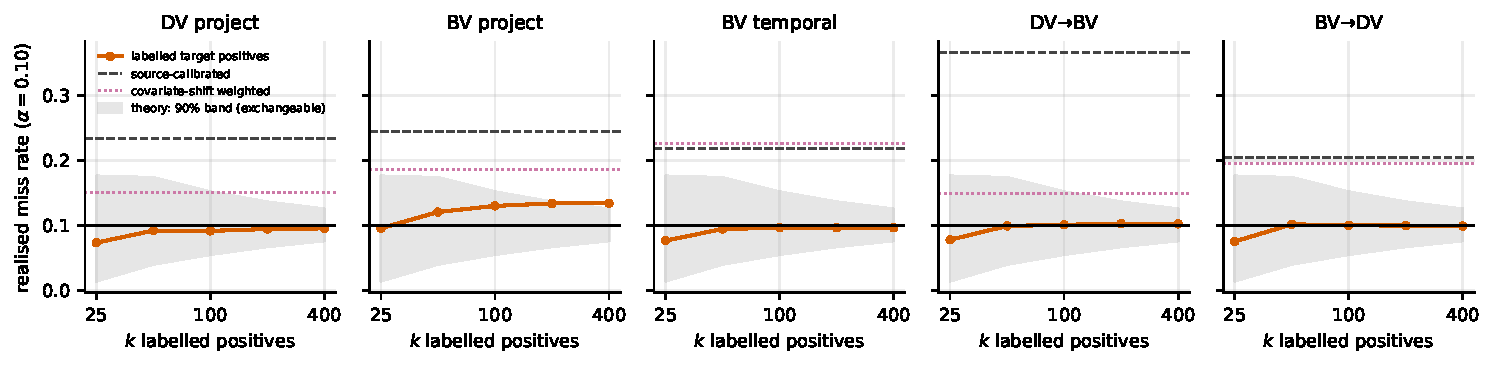
\includegraphics[width=\linewidth]{figs/fig_recalibration.pdf}
\caption{Realised miss rate at $\alpha=10\%$ as a function of the number $k$ of labelled target positives used for calibration (LR+LGBM scorer; mean over seeds). The shaded area is the 90\% band of Corollary~\ref{cor:beta} for exchangeable data; dashed and dotted lines are the source-calibrated and weighted rules.}\label{fig:recal}
\end{figure}
\begin{table}[t]
\centering\footnotesize
\caption{Conformal clearance at $\alpha{=}10\%$ (LR+LGBM scorer; all figures in \%). ID: calibrated on source data; Wtd: covariate-shift weighted; $k{=}100$: calibrated on 100 labelled target positives; PAC: $k{=}100$ with the high-probability rule ($\delta{=}0.1$) and its violation frequency $\Pr(M>\alpha+2\text{pp})$. A valid rule has miss $\lesssim10$.}\label{tab:guar}
\resizebox{\linewidth}{!}{\begin{tabular}{lccccccccc}
\toprule
Scenario & ID miss & ID SAR & Wtd miss & Wtd SAR & $k{=}100$ miss & $k{=}100$ SAR & PAC miss & PAC SAR & PAC viol. \\
\midrule
DV random & 10.1{\scriptsize$\pm$0.6} & 55.1 & -- & -- & -- & -- & -- & -- & -- \\
BV random & 8.6{\scriptsize$\pm$2.3} & 54.3 & -- & -- & -- & -- & -- & -- & -- \\
DV project & 23.6{\scriptsize$\pm$3.8} & 56.4 & 15.1 & 41.1 & 9.2 & 31.8 & 5.4 & 22.4 & 2 \\
BV project & 24.0{\scriptsize$\pm$7.6} & 47.6 & 18.6 & 34.5 & 13.0 & 28.1 & 6.9 & 15.9 & 7 \\
BV temporal & 21.7{\scriptsize$\pm$2.2} & 50.5 & 22.6 & 51.4 & 9.7 & 28.5 & 6.0 & 20.1 & 0 \\
DV$\to$BV & 37.0{\scriptsize$\pm$0.3} & 66.1 & 14.9 & 30.2 & 10.1 & 26.7 & 6.1 & 18.2 & 2 \\
BV$\to$DV & 20.3{\scriptsize$\pm$1.9} & 48.5 & 19.5 & 46.6 & 10.0 & 30.0 & 5.9 & 20.2 & 2 \\
\bottomrule
\end{tabular}}
\end{table}


\begin{figure}[t]
\centering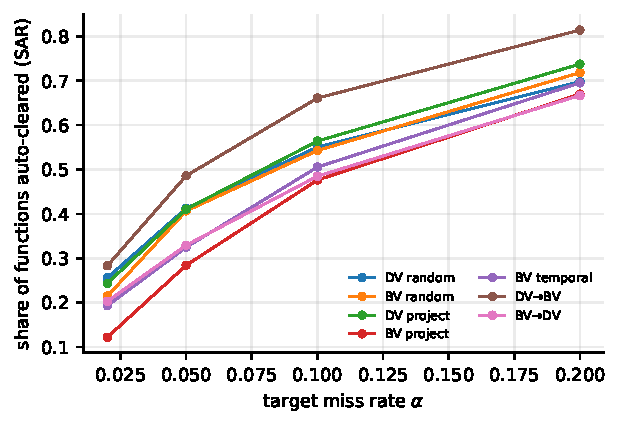
\includegraphics[width=.62\linewidth]{figs/fig_sar.pdf}
\caption{Share of functions that can be auto-cleared (SAR) versus nominal budget $\alpha$ for source-calibrated clearance (LR+LGBM). Values for shifted scenarios are \emph{not} valid; see Table~\ref{tab:guar}.}\label{fig:sar}
\end{figure}

\paragraph{Certified flagging}
Table~\ref{tab:flag} shows that the opposite decision, flagging with certified precision, offers little. With $\beta=50\%$ the Learn-then-Test procedure certifies a threshold that flags only $0.09\%$ (DiverseVul) and $2.6\%$ (Big-Vul) of the test functions on random splits (realised precision $80\%$ and $57\%$); for $\beta=70\%$ the flagged share is at most $0.3\%$ on random splits. Under shift the certification fails as well: for $\beta=50\%$, realised precision is $27\%$ (Big-Vul project), $19\%$ (Big-Vul temporal) and $23\%$ (Big-Vul$\to$DiverseVul), and the DiverseVul-trained detectors certify nothing. Learned detectors can \emph{clear} some code with a quantifiable risk, but at the precision available today they cannot be used to \emph{confirm} vulnerabilities for more than a few per cent of the code.
\begin{table}[t]
\centering\footnotesize
\caption{Certified auto-flagging (Learn-then-Test, $\delta{=}0.05$): share of test functions flagged (\%) and realised precision (\%); ``--'' = no threshold could be certified.}\label{tab:flag}
\resizebox{\linewidth}{!}{\begin{tabular}{lcccccc}
\toprule
Scenario & $\beta{=}.3$ flagged & prec. & $\beta{=}.5$ flagged & prec. & $\beta{=}.7$ flagged & prec. \\
\midrule
DV random & 1.35 & 41 & 0.09 & 80 & 0.02 & 78 \\
BV random & 8.06 & 33 & 2.57 & 57 & 0.30 & 87 \\
DV project & 0.16 & 39 & 0.00 & 43 & 0.00 & -- \\
BV project & 9.39 & 18 & 1.64 & 27 & 0.10 & 45 \\
BV temporal & 6.67 & 15 & 0.54 & 19 & 0.03 & 23 \\
DV$\to$BV & 0.33 & 56 & 0.00 & 79 & 0.00 & 75 \\
BV$\to$DV & 11.25 & 16 & 3.02 & 23 & 0.71 & 27 \\
\bottomrule
\end{tabular}}
\end{table}


\subsection{RQ4: Accountability, robustness and explanations}\label{sec:rq4}

\paragraph{The marginal guarantee is very uneven across function sizes}
Table~\ref{tab:bucket} and Figure~\ref{fig:mondrian} show that, even on exchangeable splits where the marginal guarantee holds, the miss rate at $\alpha=10\%$ is $41.4\%$ for the shortest third of DiverseVul functions and $2.2\%$ for the longest third ($25.8\%$ versus $2.9\%$ in Big-Vul). Short functions that contain vulnerabilities look like the many short benign functions, so most of the budget is consumed there. Length-conditional (Mondrian) calibration (Proposition~\ref{prop:mondrian}) equalises the three groups ($10.8/12.0/9.4\%$ in DiverseVul and $8.0/10.5/8.2\%$ in Big-Vul) at the price of a lower overall SAR ($55.2\to44.2\%$ and $54.2\to45.6\%$). Under shift it narrows the gap (e.g.\ Big-Vul project: $85.8/53.8/10.4\%\to47.3/45.4/18.1\%$) but does not restore validity, as expected, since exchangeability remains violated.

\begin{figure}[t]
\centering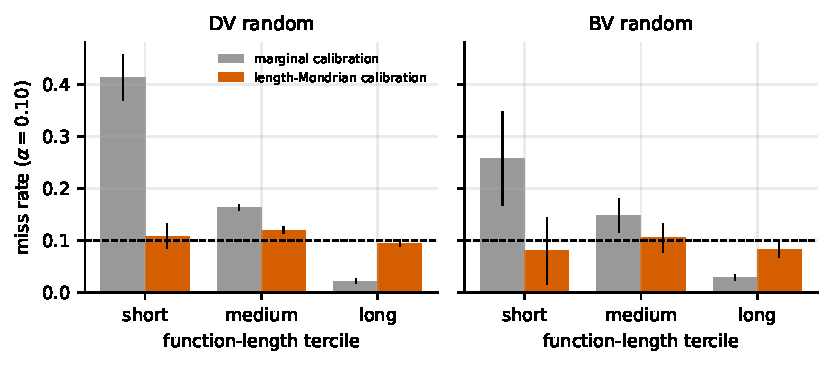
\includegraphics[width=.82\linewidth]{figs/fig_mondrian.pdf}
\caption{Miss rate per function-length tercile at $\alpha=10\%$ on random splits, marginal versus Mondrian calibration (LR+LGBM scorer, mean $\pm$ s.d.).}\label{fig:mondrian}
\end{figure}
\begin{table}[t]
\centering\footnotesize
\caption{Miss rate (\%) per function-length tercile at $\alpha{=}10\%$ for marginal (left) and Mondrian (right) calibration, with the overall share cleared (SAR). LR+LGBM scorer, ID calibration.}\label{tab:bucket}
\resizebox{\linewidth}{!}{\begin{tabular}{lcccccccc}
\toprule
Scenario & short & medium & long & SAR & short & medium & long & SAR \\
\midrule
DV random & 41.4 & 16.3 & 2.2 & 55.2 & 10.8 & 12.0 & 9.4 & 44.2 \\
BV random & 25.8 & 14.8 & 2.9 & 54.2 & 8.0 & 10.5 & 8.2 & 45.6 \\
DV project & 84.5 & 42.8 & 4.5 & 55.4 & 34.0 & 25.9 & 19.8 & 43.7 \\
BV project & 85.8 & 53.8 & 10.4 & 55.0 & 47.3 & 45.4 & 18.1 & 40.6 \\
BV temporal & 75.7 & 47.5 & 8.5 & 54.1 & 33.2 & 29.4 & 14.5 & 37.7 \\
DV$\to$BV & 90.5 & 51.3 & 7.8 & 57.1 & 37.5 & 33.5 & 29.1 & 45.2 \\
BV$\to$DV & 75.6 & 41.1 & 8.2 & 53.4 & 40.4 & 24.3 & 17.6 & 41.3 \\
\bottomrule
\end{tabular}}
\end{table}


\paragraph{Per-CWE disparity}
Figure~\ref{fig:cwe} reports miss rates per CWE for the classes with at least 15 vulnerable test functions. In DiverseVul, LightGBM misses $17.6\%$ of CWE-416 (use after free), $14.6\%$ of CWE-476 (NULL dereference) and $11.3\%$ of CWE-200, against $7.3\%$ for CWE-119, $6.8\%$ for CWE-125 and $9.1\%$ for CWE-787 (all at a nominal $10\%$); in Big-Vul the range among the most frequent classes is $2.6\%$ (CWE-125) to $14.9\%$ (CWE-264). The budget is therefore met on average but not per vulnerability class; classes that are reported separately (for audits, for example) need their own calibration, which requires sufficient labelled examples per class.
\begin{figure}[t]
\centering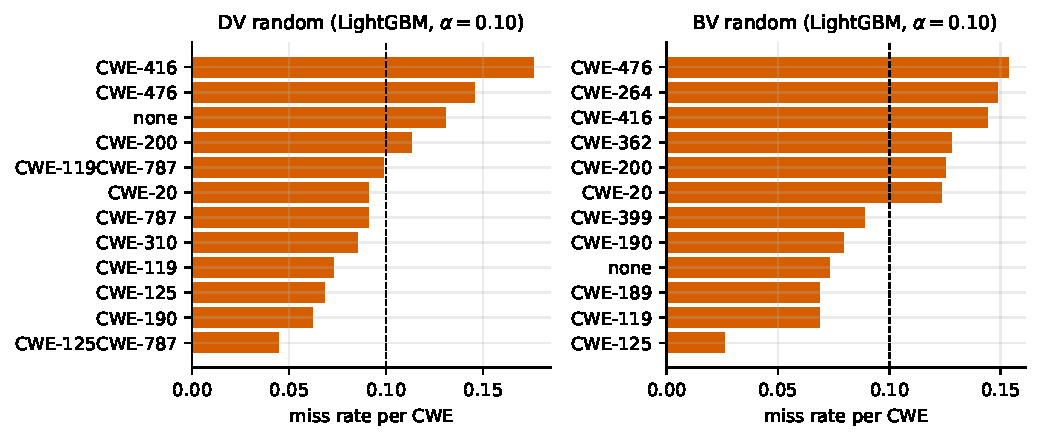
\includegraphics[width=\linewidth]{figs/fig_cwe.pdf}
\caption{Per-CWE miss rate at $\alpha=10\%$ on random splits (LightGBM, mean over seeds); the dashed line is the nominal budget.}\label{fig:cwe}
\end{figure}

\paragraph{Decision consistency under semantics-preserving rewrites}
Table~\ref{tab:robust} and Figure~\ref{fig:robust} show how the clear/review decision changes when functions are rewritten without changing behaviour. Renaming local identifiers flips $10.4\%$ of all decisions on average (and $5.6\%$ of the vulnerable functions) and inserting dead code $6.0\%$ ($2.6\%$); both together flip $13.5\%$ ($6.7\%$). The score ranking is largely preserved (Spearman $\rho=0.88$--$0.997$) and AUROC drops only by about $0.02$, but the miss rate moves from $8.6$--$11.3\%$ (original) to up to $13.5\%$ after renaming (LightGBM, DiverseVul), i.e.\ the nominal budget can be exceeded after cosmetic changes to the inputs (by $2.3$ points in the worst case, within about two points in the others). Because the triage threshold sits in the dense part of the score distribution, small score changes translate into many decision flips, which matters for accountability: the same code can be cleared or sent to review depending on variable names.
\begin{figure}[t]
\centering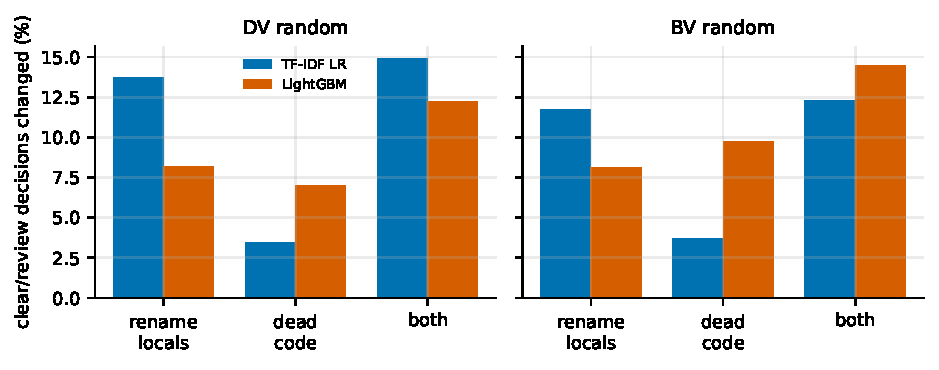
\includegraphics[width=.8\linewidth]{figs/fig_robust.pdf}
\caption{Share of clear/review decisions that change after each rewrite (5\,200 test functions per scenario, $\alpha=10\%$).}\label{fig:robust}
\end{figure}
\begin{table}[t]
\centering\footnotesize
\caption{Consistency of triage decisions ($\alpha{=}10\%$, ID calibration) on 1\,200 vulnerable and 4\,000 benign random test functions after semantics-preserving rewrites. ``Flipped'' = share of all (resp.\ vulnerable) functions whose clear/review decision changes.}\label{tab:robust}
\resizebox{\linewidth}{!}{\begin{tabular}{lllccccc}
\toprule
Scenario & Model & Rewrite & AUROC & Miss (\%) & Flipped (\%) & Flipped, vuln. (\%) & Spearman $\rho$ \\
\midrule
DV random & TF-IDF LR & original & 0.838 & 9.4 & 0.0 & 0.0 & 1.000 \\
DV random & TF-IDF LR & rename locals & 0.824 & 10.5 & 13.8 & 5.4 & 0.898 \\
DV random & TF-IDF LR & dead code & 0.837 & 8.4 & 3.5 & 1.3 & 0.997 \\
DV random & TF-IDF LR & both & 0.823 & 8.9 & 14.9 & 5.7 & 0.893 \\
DV random & LightGBM & original & 0.804 & 11.2 & 0.0 & 0.0 & 1.000 \\
DV random & LightGBM & rename locals & 0.788 & 13.5 & 8.2 & 6.8 & 0.937 \\
DV random & LightGBM & dead code & 0.800 & 9.4 & 7.0 & 3.2 & 0.978 \\
DV random & LightGBM & both & 0.785 & 10.1 & 12.2 & 8.2 & 0.917 \\
BV random & TF-IDF LR & original & 0.859 & 8.6 & 0.0 & 0.0 & 1.000 \\
BV random & TF-IDF LR & rename locals & 0.848 & 8.4 & 11.7 & 4.7 & 0.924 \\
BV random & TF-IDF LR & dead code & 0.860 & 10.5 & 3.7 & 1.9 & 0.994 \\
BV random & TF-IDF LR & both & 0.849 & 10.0 & 12.3 & 5.6 & 0.917 \\
BV random & LightGBM & original & 0.825 & 8.9 & 0.0 & 0.0 & 1.000 \\
BV random & LightGBM & rename locals & 0.810 & 10.9 & 8.1 & 5.7 & 0.937 \\
BV random & LightGBM & dead code & 0.820 & 8.3 & 9.7 & 3.9 & 0.945 \\
BV random & LightGBM & both & 0.804 & 10.0 & 14.5 & 7.2 & 0.879 \\
\bottomrule
\end{tabular}}
\end{table}


\paragraph{Explanations}
For the explanation analysis we use an interpretable LightGBM on the 71 named code metrics (Table~\ref{tab:explain}; AUROC $0.75$ on both random splits and $0.69$--$0.71$ on leak-free cross-dataset transfer, below the token-based scorers). TreeSHAP attributions are \emph{faithful} by deletion (Figure~\ref{fig:explain}, left): neutralising the ten highest-attributed features lowers the logit of the 10\% highest-scored functions by $1.63$ (DiverseVul) and $1.40$ (Big-Vul), versus $1.09$ and $0.67$ for the top-ten features by global gain and $-0.46$ and $-0.39$ for random features, so local attributions identify the features that drive the decision better than a global ranking does. They are also \emph{consistent}: the Spearman correlation of global importances is $0.97$ between training seeds and $0.90$ between a model trained on DiverseVul and one trained on Big-Vul. What they reveal is unflattering, however: the most important features are function size (characters, lines, tokens) and the number of parentheses (Figure~\ref{fig:explain}, right), i.e.\ the model largely predicts that longer, more complex functions are vulnerable. This is consistent with the length-dependent miss rate above and with the known confound that functions touched by security fixes tend to be larger. As a check on identifier shortcuts in the token model, we compared the 200 highest positive-weight lexical features of the DiverseVul logistic regression with frequency-matched random features: the former occur in a median of $11$ projects versus $13.5$ for the controls ($6\%$ versus $3\%$ occur in at most five projects), i.e.\ we do not find that the highest-weighted tokens are markedly more project-specific.
\begin{figure}[t]
\centering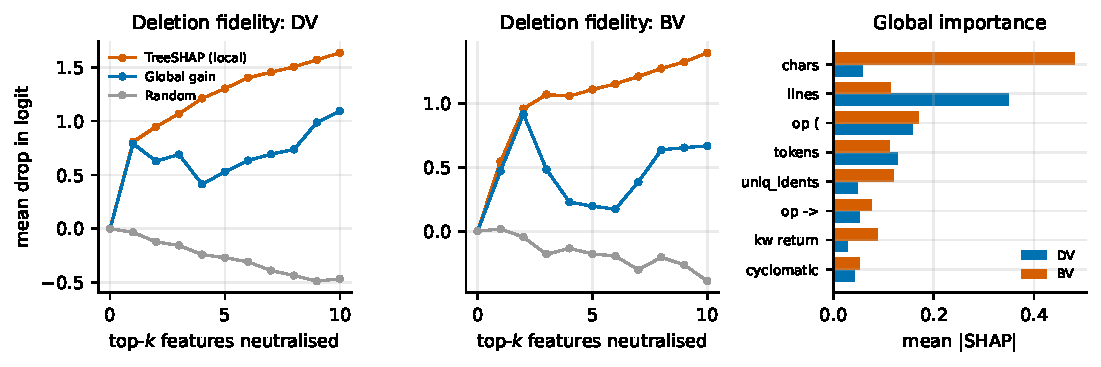
\includegraphics[width=\linewidth]{figs/fig_explain.pdf}
\caption{Explanation analysis for the metrics-only LightGBM. Left and centre: deletion fidelity (mean logit drop when the top-$k$ features of each function are neutralised). Right: mean $|$SHAP$|$ of the eight most important features.}\label{fig:explain}
\end{figure}
\begin{table}[t]
\centering\footnotesize
\caption{Interpretable metrics-only LightGBM used for the explanation analysis (3 seeds); cross-dataset rows exclude leaked functions.}\label{tab:explain}
\begin{tabular}{lcc}
\toprule
Train$\to$test & AUROC & AUPRC \\
\midrule
DV & 0.749\,{\scriptsize$\pm$0.002} & 0.164\,{\scriptsize$\pm$0.003} \\
BV & 0.756\,{\scriptsize$\pm$0.009} & 0.207\,{\scriptsize$\pm$0.012} \\
DV$\to$BV & 0.694\,{\scriptsize$\pm$0.001} & 0.132\,{\scriptsize$\pm$0.002} \\
BV$\to$DV & 0.710\,{\scriptsize$\pm$0.002} & 0.137\,{\scriptsize$\pm$0.002} \\
\bottomrule
\end{tabular}
\end{table}


\subsection{RQ5: Operational value}\label{sec:rq5}

\paragraph{Comparison with a rule-based analyser}
Flawfinder reports at least one hit for only $4.7$--$17.5\%$ of the functions and its scores barely rank the vulnerable functions (AUROC $0.535$--$0.611$, Table~\ref{tab:flaw}). Its only conservative policy, clearing functions without hits, auto-clears $82.5$--$95.3\%$ of the code but misses $62.9$--$89.8\%$ of the vulnerabilities. At the same clearance share the learned scorer misses $49.6$--$81.3\%$, and for the same (high) miss rate it could clear $84.7$--$98.8\%$ (Figure~\ref{fig:flaw}). Neither is useful as an unattended filter at those operating points; the contrast is that the learned scorer provides a whole curve from which a budget such as $10\%$ can be chosen and certified, whereas Flawfinder provides a single, uncontrolled point.
\begin{figure}[t]
\centering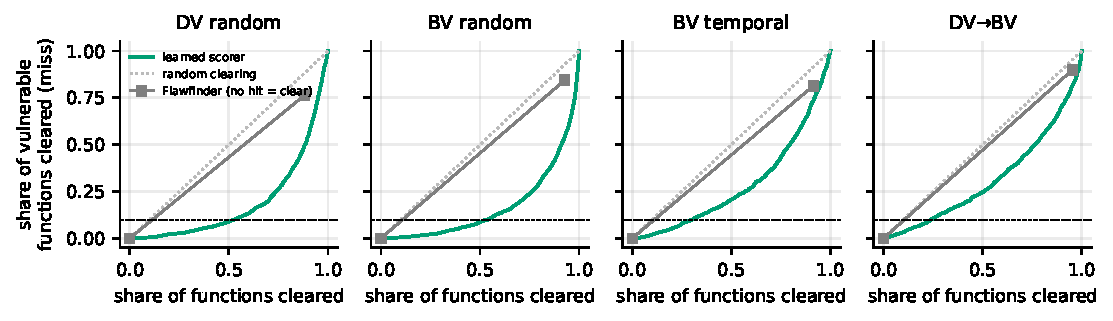
\includegraphics[width=\linewidth]{figs/fig_flaw.pdf}
\caption{Miss rate versus share of functions cleared for the learned scorer (curve) and Flawfinder (square; ``no hit $=$ clear''). Dashed: $10\%$ budget; dotted: random clearing.}\label{fig:flaw}
\end{figure}
\begin{table}[t]
\centering\footnotesize
\caption{Flawfinder (FF) versus the learned scorer (LR+LGBM rank average) on identical test functions (seed 0). The only conservative FF policy is to clear functions without any hit; its SAR and miss rate (\%) are compared with the learned scorer's miss rate at the same SAR and its SAR at the same miss rate.}\label{tab:flaw}
\resizebox{\linewidth}{!}{\begin{tabular}{lcccccccc}
\toprule
Scenario & AUROC FF & AUROC ML & AUPRC FF & AUPRC ML & FF SAR & FF miss & ML miss @SAR & ML SAR @miss \\
\midrule
DV random & 0.570 & 0.830 & 0.075 & 0.230 & 88.3 & 76.4 & 49.6 & 95.4 \\
BV random & 0.548 & 0.851 & 0.065 & 0.380 & 92.7 & 84.4 & 54.4 & 98.8 \\
DV project & 0.568 & 0.709 & 0.070 & 0.126 & 90.6 & 79.7 & 71.8 & 94.3 \\
BV project & 0.611 & 0.700 & 0.101 & 0.141 & 82.5 & 62.9 & 58.9 & 84.7 \\
BV temporal & 0.555 & 0.726 & 0.058 & 0.110 & 91.4 & 81.3 & 73.3 & 94.7 \\
DV$\to$BV & 0.535 & 0.697 & 0.066 & 0.163 & 95.3 & 89.8 & 81.3 & 98.4 \\
BV$\to$DV & 0.570 & 0.707 & 0.079 & 0.141 & 88.3 & 77.2 & 68.1 & 92.7 \\
\bottomrule
\end{tabular}}
\end{table}


\paragraph{Economic view}
Table~\ref{tab:cost} and Figure~\ref{fig:cost} apply the cost model of Eq.~\eqref{eq:cost} with $\alpha^\star$ chosen on ID calibration data. On random splits and for a missed vulnerability that costs $50$ reviews, the optimal budget is $\alpha^\star=0.07$--$0.09$, the rule clears $48$--$53\%$ of the code, and expected cost is $0.68$--$0.73$ of reviewing everything. Under project, temporal and cross-dataset shift the same procedure yields costs of $0.95$--$1.27$, i.e.\ no saving or a loss, because the miss rate it believes to have ($\approx\alpha^\star$) is far from the realised one. For $c_m=10$, triage appears to save $46$--$69\%$ of the cost but misses $35$--$75\%$ of the vulnerabilities, and for $c_m=200$ the saving is only $4$--$6\%$ on random splits and negative under shift; for $c_m=1000$ ``review everything'' is optimal in all scenarios. In short: delegation pays when a miss is worth tens, not hundreds, of reviews, and only if the miss rate is calibrated on the deployment distribution.
\begin{figure}[t]
\centering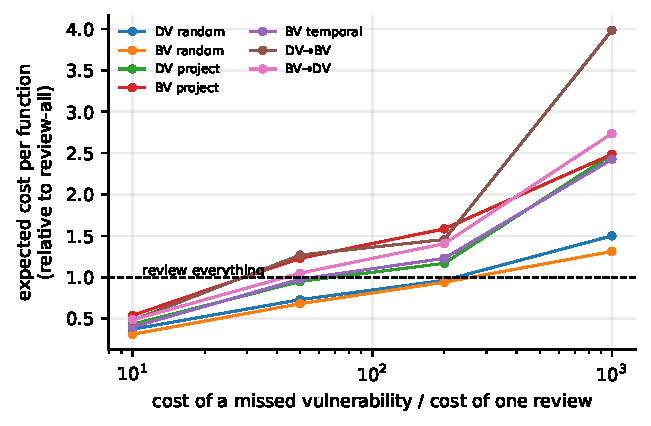
\includegraphics[width=.62\linewidth]{figs/fig_cost.pdf}
\caption{Expected cost per function relative to reviewing everything as a function of the cost ratio $c_m$ (LR+LGBM, $\alpha^\star$ selected on ID calibration data).}\label{fig:cost}
\end{figure}
\begin{table}[t]
\centering\footnotesize
\caption{Cost-optimal miss budget $\alpha^\star$ chosen on ID calibration data, its realised SAR (\%) and expected cost per function relative to reviewing everything ($=1$), for $c_m=10$, $50$, $200$ review units per missed vulnerability. LR+LGBM scorer.}\label{tab:cost}
\resizebox{\linewidth}{!}{\begin{tabular}{lccccccccc}
\toprule
Scenario & $\alpha^\star$ & SAR & cost & $\alpha^\star$ & SAR & cost & $\alpha^\star$ & SAR & cost \\
\midrule
DV random & 0.35 & 82 & 0.37 & 0.07 & 48 & 0.73 & 0.01 & 17 & 0.96 \\
BV random & 0.43 & 90 & 0.31 & 0.09 & 53 & 0.68 & 0.01 & 15 & 0.94 \\
DV project & 0.33 & 86 & 0.43 & 0.06 & 46 & 0.95 & 0.01 & 16 & 1.17 \\
BV project & 0.37 & 85 & 0.54 & 0.09 & 46 & 1.23 & 0.02 & 11 & 1.59 \\
BV temporal & 0.38 & 89 & 0.40 & 0.11 & 53 & 0.98 & 0.01 & 16 & 1.23 \\
DV$\to$BV & 0.38 & 93 & 0.48 & 0.08 & 62 & 1.27 & 0.01 & 17 & 1.46 \\
BV$\to$DV & 0.35 & 83 & 0.49 & 0.08 & 45 & 1.05 & 0.02 & 18 & 1.41 \\
\bottomrule
\end{tabular}}
\end{table}


\subsection{RQ6: Pre-trained code model and shortcut learning}\label{sec:rq6}
Tables~\ref{tab:cbdetect} and~\ref{tab:cbtriage} and Figure~\ref{fig:cb} report the CodeBERT experiment on the 30\,000-function subsample (Section~\ref{sec:design_cb}).

\paragraph{Raw text rewards a dataset artifact}
With raw text as input, CodeBERT looks excellent on Big-Vul: the CodeBERT ensemble reaches AUROC $0.893$ (random), $0.828$ (project) and $0.844$ (temporal), against $0.825$, $0.709$ and $0.728$ for the TF-IDF+LightGBM scorer trained on the same subsample. The formatting-only classifier (the 15 statistics above, of which whitespace structure alone carries most of the signal on Big-Vul) does even better ($0.924$, $0.895$, $0.909$; AUPRC $0.59$--$0.65$ against $0.12$--$0.25$ for the lexical scorers), and the advantage does not transfer: on DiverseVul the formatting-only classifier reaches $0.730$ (random) and $0.690$ (project), and Big-Vul$\to$DiverseVul falls to $0.627$ (Table~\ref{tab:cbdetect}). The artifact is visible in the data (Table~\ref{tab:format}): $3.0\%$ of the lines of vulnerable Big-Vul functions end in whitespace against $0.1\%$ of benign ones, $24.3\%$ versus $6.5\%$ of the functions start with whitespace, and vulnerable functions contain $2.9$ comment markers on average against $0.8$. It is much weaker in DiverseVul, which has other, smaller differences (comment markers $5.3$ versus $1.8$). When the same CodeBERT is given normalised text, its Big-Vul AUROC drops by $0.12$ in all three scenarios ($0.774$, $0.706$, $0.721$) while DiverseVul is unchanged ($0.753$ and $0.702$ versus $0.745$ and $0.698$).

\paragraph{Frozen CodeBERT adds little on normalised text}
Without the artifact, the CodeBERT ensemble is below the lexical scorer on random splits ($0.753$ vs.\ $0.790$ on DiverseVul, $0.774$ vs.\ $0.825$ on Big-Vul) and level under shift ($0.689$--$0.721$ vs.\ $0.701$--$0.728$). Combining the two (TF-IDF+CodeBERT) is the best normalised scorer in every shifted scenario, but by only $0.002$--$0.010$ AUROC (AUPRC $0.123$--$0.154$ vs.\ $0.115$--$0.148$). Frozen general-purpose embeddings thus do not change the picture of Section~\ref{sec:rq1}, and neither does fine-tuning (next paragraph).

\paragraph{Fine-tuning does not change the picture} Table~\ref{tab:ft} compares end-to-end fine-tuned CodeBERT (validation AUROC $0.76$--$0.83$) with the other scorers on exactly the same scenario--seed pairs (one or two seeds per scenario). Fine-tuning does not improve on the frozen embeddings (AUROC between $-0.015$ and $+0.009$ relative to the frozen ensemble) and stays $0.004$--$0.040$ below the lexical ensemble; combining it with the lexical scorers adds $0.000$--$0.015$ over the lexical ensemble alone. The triage findings are unchanged: with source calibration the realised miss rate at $\alpha=10\%$ is $10.9\%$ on the random splits (DiverseVul $10.4\%$, Big-Vul $11.5\%$, within the roughly one-point sampling error of one or two seeds) and $13.8\%$ on average over the shifted scenarios, from $10.2\%$ (Big-Vul project) to $20.7\%$ (DiverseVul$\to$Big-Vul), against $16.2\%$ for the lexical scorer and $14.6\%$ for frozen CodeBERT on the same pairs; recalibration on 100 labelled target positives restores $8.7$--$11.5\%$ at a SAR of $23$--$29\%$, and all $33$ observations satisfy the KS bound. The levels of automation that can be validly delegated are therefore driven by the shift and by the amount of labelled target data, not by the choice among these scorers.

\begin{figure}[t]
\centering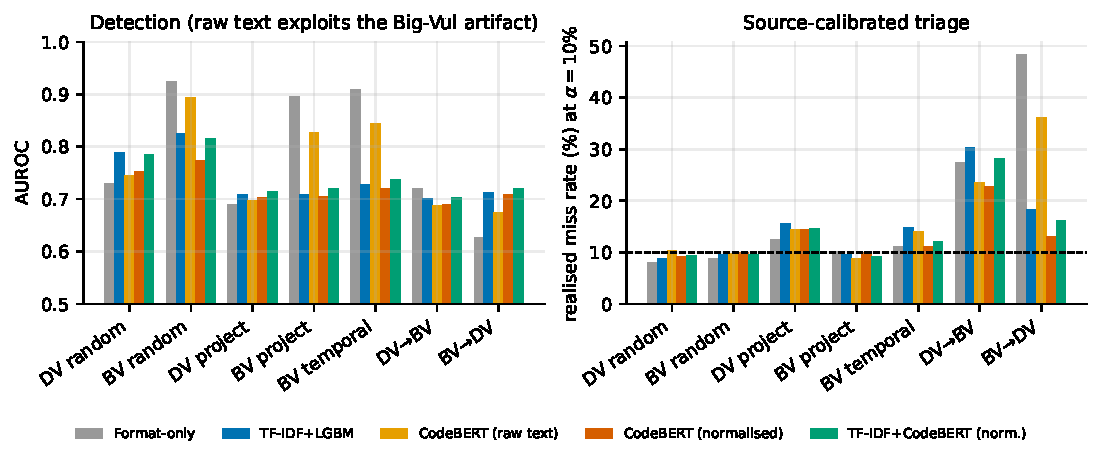
\includegraphics[width=\linewidth]{figs/fig_cb.pdf}
\caption{Left: AUROC of the formatting-only probe, the TF-IDF+LightGBM scorer and the CodeBERT scorers (raw and normalised text) on the subsample. Right: realised miss rate at $\alpha=10\%$ when calibrated on source data (dashed: nominal).}\label{fig:cb}
\end{figure}
\begin{table}[t]
\centering\footnotesize
\caption{Detection with frozen CodeBERT embeddings on the stratified subsample (mean over 3 seeds; AUPRC weighted to the true prevalence). Fmt: formatting-only classifier; CB raw / norm: CodeBERT on raw text / on comment-and-whitespace-normalised text; ensembles are standardised score sums.}\label{tab:cbdetect}
\resizebox{\linewidth}{!}{\begin{tabular}{lcccccccccc}
\toprule
Scenario & AUROC Fmt & AUROC TF-IDF & AUROC CB raw & AUROC CB norm & AUROC TF+CB & AUPRC Fmt & AUPRC TF-IDF & AUPRC CB raw & AUPRC CB norm & AUPRC TF+CB \\
\midrule
DV random & 0.730 & 0.790 & 0.745 & 0.753 & 0.784 & 0.143 & 0.208 & 0.168 & 0.167 & 0.203 \\
BV random & 0.924 & 0.825 & 0.893 & 0.774 & 0.816 & 0.651 & 0.251 & 0.445 & 0.180 & 0.240 \\
DV project & 0.690 & 0.708 & 0.698 & 0.702 & 0.715 & 0.122 & 0.137 & 0.122 & 0.135 & 0.147 \\
BV project & 0.895 & 0.709 & 0.828 & 0.706 & 0.719 & 0.588 & 0.142 & 0.312 & 0.142 & 0.152 \\
BV temporal & 0.909 & 0.728 & 0.844 & 0.721 & 0.737 & 0.647 & 0.115 & 0.291 & 0.121 & 0.123 \\
DV$\to$BV & 0.720 & 0.701 & 0.688 & 0.689 & 0.703 & 0.193 & 0.148 & 0.126 & 0.139 & 0.154 \\
BV$\to$DV & 0.627 & 0.712 & 0.674 & 0.709 & 0.721 & 0.101 & 0.147 & 0.113 & 0.140 & 0.153 \\
\bottomrule
\end{tabular}}
\end{table}

\begin{table}[t]
\centering\footnotesize
\caption{Fine-tuned CodeBERT on normalised text compared with the other scorers on exactly the same (scenario, seed) pairs (seed 0 for all scenarios, seed 1 additionally for BV-R, BV-P, BV-T and DV-R; the other models in Tables~\ref{tab:cbdetect} and~\ref{tab:cbtriage} use three seeds). AUROC, AUPRC (weighted to true prevalence) and realised miss rate (\%) of source-calibrated clearance at $\alpha{=}10\%$.}\label{tab:ft}
\resizebox{\linewidth}{!}{\begin{tabular}{lcccccccccccccc}
\toprule
Scenario & Seeds & AUROC TF-IDF+LGBM & AUROC CB frozen & AUROC CB fine-tuned & AUROC TF+CB-FT & AUPRC TF-IDF+LGBM & AUPRC CB frozen & AUPRC CB fine-tuned & AUPRC TF+CB-FT & miss TF-IDF+LGBM & miss CB frozen & miss CB fine-tuned & miss TF+CB-FT \\
\midrule
DV random & 2 & 0.787 & 0.754 & 0.747 & 0.787 & 0.200 & 0.169 & 0.163 & 0.202 & 8.9 & 9.4 & 10.4 & 9.2 \\
BV random & 2 & 0.827 & 0.780 & 0.789 & 0.833 & 0.250 & 0.181 & 0.208 & 0.266 & 9.5 & 9.4 & 11.5 & 10.6 \\
DV project & 1 & 0.716 & 0.702 & 0.692 & 0.722 & 0.136 & 0.134 & 0.118 & 0.140 & 14.3 & 13.3 & 18.5 & 14.6 \\
BV project & 2 & 0.693 & 0.687 & 0.689 & 0.708 & 0.134 & 0.135 & 0.129 & 0.140 & 11.7 & 13.6 & 10.2 & 10.6 \\
BV temporal & 2 & 0.728 & 0.720 & 0.723 & 0.739 & 0.115 & 0.117 & 0.115 & 0.123 & 14.4 & 11.0 & 11.0 & 13.4 \\
DV$\to$BV & 1 & 0.699 & 0.689 & 0.691 & 0.711 & 0.150 & 0.139 & 0.130 & 0.155 & 29.3 & 26.0 & 20.7 & 27.0 \\
BV$\to$DV & 1 & 0.712 & 0.711 & 0.696 & 0.720 & 0.146 & 0.135 & 0.128 & 0.149 & 18.0 & 13.5 & 14.7 & 18.9 \\
\bottomrule
\end{tabular}}
\end{table}

\begin{table}[t]
\centering\footnotesize
\caption{Formatting-shortcut audit on the stratified subsample (random 70/30 split). First two columns: LightGBM on 15 formatting features of the raw text only (indentation, trailing whitespace, comment markers, line lengths; AUPRC weighted to true prevalence). Next three: mean per function, vulnerable / benign. Last: AUROC of the main-study LightGBM with all metrics / with size-sensitive metrics (chars, lines, tokens) removed (seed 0).}\label{tab:format}
\resizebox{\linewidth}{!}{\begin{tabular}{lcccccc}
\toprule
Dataset & AUROC & AUPRC & Trailing-ws lines (\%) & Starts with ws (\%) & Comment markers & Main LGBM AUROC \\
\midrule
Big-Vul & 0.919 & 0.643 & 3.0 / 0.1 & 24.3 / 6.5 & 2.9 / 0.8 & 0.820 / 0.818 \\
DiverseVul & 0.721 & 0.145 & 0.5 / 0.2 & 4.2 / 7.9 & 5.3 / 1.8 & 0.801 / 0.802 \\
\bottomrule
\end{tabular}}
\end{table}


\paragraph{The guarantee findings replicate}
For every CodeBERT-based scorer the realised miss rate at $\alpha=10\%$ is on target on random splits (CodeBERT ensemble $9.6\%$ normalised, $10.0\%$ raw; TF-IDF $9.2\%$; combined $9.5\%$) and exceeded under shift (averages over the five shifted scenarios: $14.3\%$ normalised CodeBERT, $19.4\%$ raw CodeBERT, $17.7\%$ TF-IDF, $16.0\%$ combined; Table~\ref{tab:cbtriage}), and all $504$ (normalised) and $441$ (raw) observations satisfy the KS bound of Proposition~\ref{prop:shift}. Calibrating on 100 labelled target positives restores the budget for every scorer (mean miss $9.1$--$9.6\%$, range $7.5$--$10.1\%$ over scenarios), and the PAC variant keeps the violation frequency at or below $1.3\%$. The excess under shift is smaller than in the main study ($1.4$--$1.9\times$ against $2.7\times$) because of the smaller training sets and, above all, because the project partitions of the subsample are milder (see Section~\ref{sec:rq3}); the cross-dataset violation remains large ($22.7$--$30.4\%$ for DiverseVul$\to$Big-Vul).

\paragraph{A scorer can be valid and efficient for the wrong reason}
The shortcut scorers are the most efficient. Calibrated on 100 target positives, the formatting-only probe clears $62.4\%$ and $54.5\%$ of Big-Vul functions under project and temporal shift, and raw-text CodeBERT $53.8\%$ and $53.7\%$, against $27$--$32\%$ for the lexical scorers and $26.9$ and $26.1\%$ for normalised CodeBERT; within Big-Vul the formatting-only probe meets its budget with source calibration (miss $10.2\%$ and $11.1\%$ under project and temporal shift) and raw CodeBERT nearly so ($8.9\%$ and $14.0\%$). The same scorers break the moment the shortcut does not hold: calibrated on Big-Vul and applied to DiverseVul they miss $48.4\%$ (formatting-only) and $36.2\%$ (raw CodeBERT) of the vulnerabilities at a $10\%$ budget, against $13.0\%$ for normalised CodeBERT and $18.3\%$ for the lexical scorer. A conformal guarantee is a statement about the calibration distribution; it says nothing about whether the score separates vulnerabilities for a reason that survives deployment. This is one more reason to audit inputs for shortcuts and to calibrate on data from the deployment distribution.
\begin{table}[t]
\centering\footnotesize
\caption{Triage with CodeBERT scorers at $\alpha{=}10\%$ (\%). Left: realised miss rate when calibrated on source (ID) data; right: safe automation rate when calibrated on 100 labelled target positives (valid by Prop.~\ref{prop:valid}). Subsample experiment; see Table~\ref{tab:cbdetect} for column keys.}\label{tab:cbtriage}
\resizebox{\linewidth}{!}{\begin{tabular}{lcccccccccc}
\toprule
Scenario & miss Fmt & miss TF-IDF & miss CB raw & miss CB norm & miss TF+CB & SAR Fmt & SAR TF-IDF & SAR CB raw & SAR CB norm & SAR TF+CB \\
\midrule
DV random & 8.0 & 8.8 & 10.3 & 9.2 & 9.4 & -- & -- & -- & -- & -- \\
BV random & 8.9 & 9.6 & 9.7 & 10.0 & 9.5 & -- & -- & -- & -- & -- \\
DV project & 12.6 & 15.6 & 14.5 & 14.4 & 14.6 & 24.7 & 26.8 & 24.9 & 25.6 & 28.1 \\
BV project & 10.2 & 9.5 & 8.9 & 10.1 & 9.2 & 62.7 & 32.1 & 53.8 & 27.0 & 29.6 \\
BV temporal & 11.1 & 14.9 & 14.0 & 11.2 & 12.1 & 54.7 & 27.4 & 53.7 & 25.0 & 27.3 \\
DV$\to$BV & 27.4 & 30.4 & 23.6 & 22.7 & 28.1 & 17.1 & 24.7 & 23.4 & 24.2 & 24.5 \\
BV$\to$DV & 48.4 & 18.3 & 36.2 & 13.0 & 16.1 & 14.7 & 28.9 & 24.2 & 29.1 & 31.0 \\
\midrule
Mean, random & 8.4 & 9.2 & 10.0 & 9.6 & 9.5 &  &  &  &  &  \\
Mean, shifted & 21.9 & 17.7 & 19.4 & 14.3 & 16.0 & 34.8 & 28.0 & 36.0 & 26.2 & 28.1 \\
\bottomrule
\end{tabular}}
\end{table}


\subsection{RQ7: Online calibration under drift}\label{sec:rq7}
Table~\ref{tab:online} and Figure~\ref{fig:online} show the effect of replaying the test sets as streams at $\alpha=10\%$.
\paragraph{Static calibration drifts out of budget.} The fixed threshold misses $21.7\%$ (Big-Vul temporal), $24.0\%$ and $23.6\%$ (Big-Vul and DiverseVul project streams), $37.0\%$ (DiverseVul$\to$Big-Vul) and $20.3\%$ (Big-Vul$\to$DiverseVul) of the vulnerable functions over the stream. Its worst window is worse still ($27$--$45\%$): in the temporal stream the rolling miss rate stays between $15$ and $35\%$ for the whole period (Figure~\ref{fig:online}, left), so the violation is not a transient at the start.
\paragraph{ACI restores the long-run budget with delayed feedback only.} With $\gamma=0.01$ the overall miss rate is $10.2\%$, $10.1\%$, $10.2\%$ and $10.1\%$ on the temporal, DiverseVul project, DiverseVul$\to$Big-Vul and Big-Vul$\to$DiverseVul streams and $11.5\%$ on the Big-Vul project stream, where abrupt project switches are the hardest case. The deterministic bound of Proposition~\ref{prop:online} holds in all $168$ runs (Table~\ref{tab:gamma}; it is conservative, about $9$ points on average at $\gamma=0.01$, while the observed deviations are at most $3$ points). Worst-window miss rates fall to $13$--$19\%$. The sliding-window recalibration is comparable but somewhat worse in overall miss ($9.8$--$13.1\%$) and needs stored target scores; combining it with ACI gives the closest match to the budget ($9.9$--$11.3\%$).
\paragraph{The price is automation, and it is the valid level.} Under shift ACI ($\gamma=0.01$) clears $22$--$29\%$ of the functions (static: $48$--$66\%$, but invalid), in line with the $27$--$32\%$ obtained by one-off recalibration with 100 labelled target positives in Section~\ref{sec:rq3}. On the stationary random streams ACI clears $54.0\%$ and $56.9\%$ at $10.0\%$ and $9.9\%$ miss, as the static rule does ($55.1\%$, $54.3\%$): adaptation does no harm where there is no drift. Large steps are counter-productive: $\gamma=0.05$ keeps the budget but reduces SAR by $4$--$16$ points relative to $\gamma=0.01$, because its level oscillates; $\gamma\in[0.005,0.01]$ was best here.
\begin{figure}[t]
\centering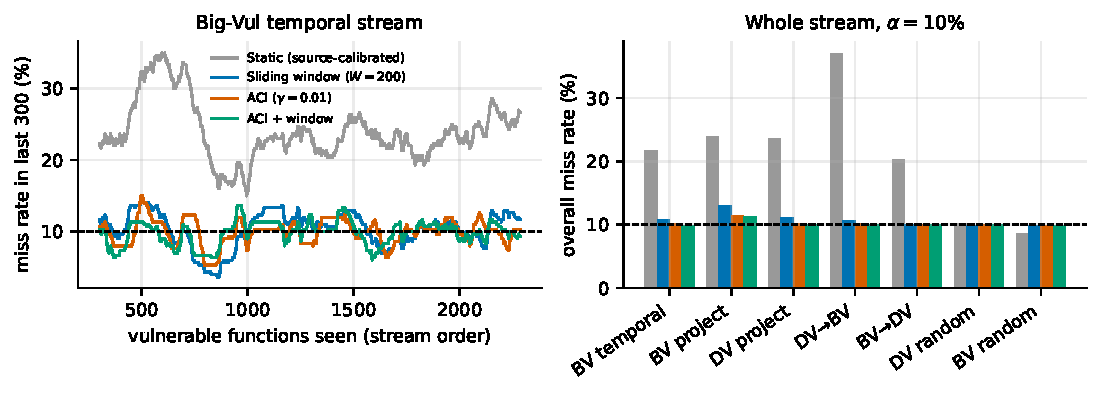
\includegraphics[width=\linewidth]{figs/fig_online.pdf}
\caption{Left: miss rate over the last 300 vulnerable functions along the Big-Vul temporal stream (seed 0, $\alpha=10\%$). Right: overall miss rate of each stream for the four policies (mean over 3 seeds).}\label{fig:online}
\end{figure}
\begin{table}[t]
\centering\footnotesize
\caption{Online risk control at $\alpha{=}10\%$ on arrival-ordered test streams (batches of 1\,000 functions, labels revealed after each batch; LR+LGBM scorer; mean over 3 seeds, \%). Overall miss rate over the stream, worst miss rate in any window of 300 vulnerable functions, and share of functions cleared (SAR). Static: threshold fixed from source calibration; SW: recalibrated on the last 200 observed vulnerable functions; ACI: adaptive conformal inference with step $\gamma$; ACI+window: ACI on the sliding-window reference.}\label{tab:online}
\resizebox{\linewidth}{!}{\begin{tabular}{lcccccccccccc}
\toprule
& \multicolumn{4}{c}{overall miss} & \multicolumn{4}{c}{worst window miss} & \multicolumn{4}{c}{SAR} \\
\cmidrule(lr){2-5}\cmidrule(lr){6-9}\cmidrule(lr){10-13}
Stream & Static & SW & ACI & ACI+W & Static & SW & ACI & ACI+W & Static & SW & ACI & ACI+W \\
\midrule
BV temporal & 21.7 & 10.8 & 10.2 & 9.9 & 32.8 & 15.9 & 13.8 & 14.1 & 50.5 & 30.2 & 29.2 & 27.3 \\
BV project & 24.0 & 13.1 & 11.5 & 11.3 & 30.0 & 16.7 & 17.0 & 16.7 & 47.6 & 28.3 & 22.4 & 22.7 \\
DV project & 23.6 & 11.2 & 10.1 & 10.0 & 33.8 & 17.7 & 18.7 & 19.2 & 56.4 & 34.4 & 29.4 & 27.1 \\
DV$\to$BV & 37.0 & 10.7 & 10.2 & 10.0 & 45.1 & 17.3 & 13.2 & 13.1 & 66.1 & 27.5 & 24.2 & 25.4 \\
BV$\to$DV & 20.3 & 10.0 & 10.1 & 10.0 & 27.0 & 16.0 & 13.0 & 13.1 & 48.5 & 30.2 & 29.1 & 28.5 \\
DV random & 10.1 & 9.8 & 10.0 & 10.0 & 14.1 & 13.3 & 13.1 & 13.1 & 55.1 & 53.7 & 53.9 & 49.7 \\
BV random & 8.6 & 9.8 & 9.9 & 9.9 & 11.2 & 12.9 & 12.7 & 12.9 & 54.3 & 57.3 & 56.9 & 52.8 \\
\bottomrule
\end{tabular}}
\end{table}

\begin{table}[t]
\centering\footnotesize
\caption{Sensitivity of ACI to the step size $\gamma$ ($\alpha{=}10\%$): overall miss, the deterministic bound $(1+\gamma b)/(\gamma N)$ of Proposition~\ref{prop:online} on its deviation from $\alpha$ (\%), SAR and worst-window miss.}\label{tab:gamma}
\begin{tabular}{lccccc}
\toprule
Stream & $\gamma$ & miss & bound & SAR & worst window \\
\midrule
BV temporal & 0.005 & 10.4 & 13.7 & 30.2 & 14.0 \\
BV temporal & 0.01 & 10.2 & 9.4 & 29.2 & 13.8 \\
BV temporal & 0.02 & 10.1 & 7.2 & 25.7 & 14.1 \\
BV temporal & 0.05 & 10.1 & 5.9 & 20.3 & 17.4 \\
BV project & 0.005 & 11.9 & 32.5 & 22.6 & 13.8 \\
BV project & 0.01 & 11.5 & 22.3 & 22.4 & 17.0 \\
BV project & 0.02 & 11.4 & 17.3 & 22.8 & 17.6 \\
BV project & 0.05 & 11.9 & 14.2 & 18.3 & 22.6 \\
DV$\to$BV & 0.005 & 10.4 & 6.5 & 26.0 & 15.2 \\
DV$\to$BV & 0.01 & 10.2 & 4.1 & 24.2 & 13.2 \\
DV$\to$BV & 0.02 & 10.2 & 2.9 & 20.6 & 15.6 \\
DV$\to$BV & 0.05 & 10.2 & 2.2 & 16.6 & 18.4 \\
\bottomrule
\end{tabular}
\end{table}


\subsection{RQ8: Replication on a third corpus (PrimeVul)}\label{sec:rq8}
\paragraph{Audit} PrimeVul contains 222\,558 clean functions (2.5\% vulnerable, 753 projects; Table~\ref{tab:data3}). It is not independent of the other two corpora: $77.3\%$ of its functions (171\,951) also occur in DiverseVul and $35.6\%$ (79\,323) in Big-Vul, including 4\,606 of its 5\,648 vulnerable functions that occur in DiverseVul. A cross-dataset evaluation between these corpora that does not remove shared functions would therefore mostly measure memorisation; all our cross-dataset scenarios do remove them.
\begin{table}[t]
\centering\footnotesize
\caption{Three corpora after normalisation and de-duplication. Pairwise overlaps of normalised functions: DiverseVul$\cap$Big-Vul 69,268 (42.7\% of Big-Vul), PrimeVul$\cap$DiverseVul 171,951 (77.3\% of PrimeVul), PrimeVul$\cap$Big-Vul 79,323 (35.6\% of PrimeVul).}\label{tab:data3}
\begin{tabular}{lrrrrr}
\toprule
Corpus & Raw & Exact duplicates & Clean & Vulnerable & Projects \\
\midrule
DiverseVul & 328,907 & 3,025 & 325,138 & 17,689 (5.4\%) & 800 \\
Big-Vul & 216,568 & 53,373 & 162,274 & 8,055 (5.0\%) & 309 \\
PrimeVul & 223,335 & 725 & 222,558 & 5,648 (2.5\%) & 753 \\
\bottomrule
\end{tabular}
\end{table}

\paragraph{Detection} With the same detectors (Table~\ref{tab:pv}), PrimeVul is the hardest corpus in absolute terms: AUROC $0.840$ and AUPRC $0.139$ on a random split ($5.5\times$ the prevalence of $2.5\%$), falling to $0.797$ and $0.111$ for held-out projects, $0.819$ and $0.114$ for later CVEs, and $0.715$--$0.826$ across the cross-dataset scenarios.
\paragraph{The guarantee replicates} On the random split the source-calibrated rule misses $10.7\%$ at $\alpha=10\%$. Under shift it misses more in all six scenarios: $11.8\%$ (temporal, the mildest), $13.2\%$ (DiverseVul$\to$PrimeVul), $14.0\%$ (Big-Vul$\to$PrimeVul), $19.0\%$ (project; $15.5$--$22.0\%$ across partitions), $23.9\%$ (PrimeVul$\to$DiverseVul) and $36.1\%$ (PrimeVul$\to$Big-Vul); the average over the shifted scenarios is $19.7\%$, i.e.\ $2.0\times$ the budget, and all $336$ observations satisfy the KS bound of Proposition~\ref{prop:shift}. Temporal shift is much less harmful here than on Big-Vul ($11.8$ against $21.7\%$), which shows that the size of the violation depends on the corpus and the split and cannot be inferred in advance. Covariate-shift weighting nearly restores the budget in three scenarios (project $19.0\to12.1\%$, temporal $11.8\to10.7\%$, DiverseVul$\to$PrimeVul $13.2\to10.6\%$), halves the excess for PrimeVul$\to$Big-Vul ($36.1\to19.5\%$) and does nothing for Big-Vul$\to$PrimeVul and PrimeVul$\to$DiverseVul ($14.1\%$, $23.1\%$): it is more useful here than on the other corpora but still not reliable. With 100 labelled target positives the realised miss rate is $8.7$--$10.7\%$ in every scenario, at a SAR of $25.9$--$50.8\%$ (PAC variant: $17.8$--$39.1\%$, violation frequency $\le4.5\%$ in all scenarios).
\paragraph{Shortcut} The raw-text formatting probe reaches AUROC $0.883$ on PrimeVul, of which whitespace structure alone gives $0.841$ and size alone $0.805$ (Table~\ref{tab:formatabl}); the scorers of this paper ignore whitespace, and removing the size-sensitive metrics changes the PrimeVul LightGBM AUROC by at most $0.006$. We did not trace the origin of the PrimeVul signal: because many benign functions are patched twins of vulnerable ones, formatting differences may reflect how the fixes were applied.
\begin{figure}[t]
\centering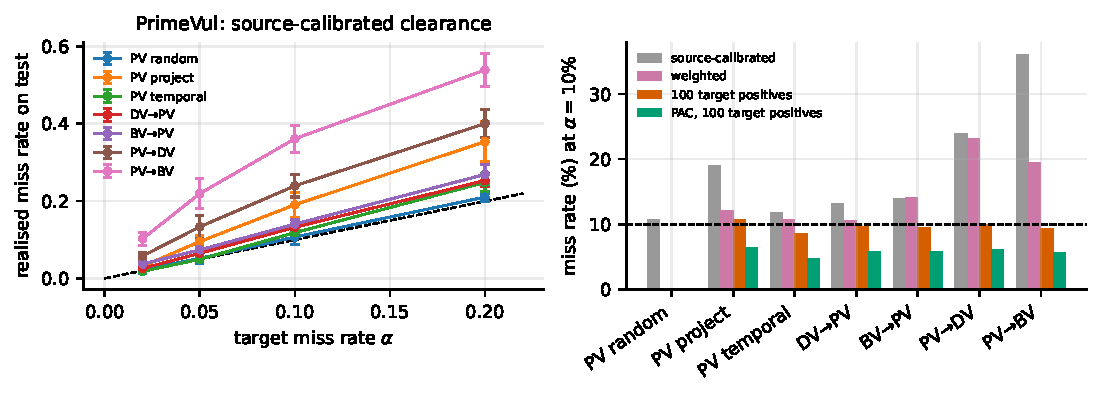
\includegraphics[width=\linewidth]{figs/fig_pv.pdf}
\caption{PrimeVul. Left: realised versus nominal miss rate of source-calibrated clearance (mean $\pm$ s.d.). Right: miss rate at $\alpha=10\%$ for source calibration, covariate-shift weighting and recalibration on 100 target positives (plain and PAC).}\label{fig:pv}
\end{figure}
\begin{table}[t]
\centering\footnotesize
\caption{Replication on PrimeVul (LR+LGBM scorer, mean over 3 seeds; \%, except AUROC/AUPRC). ID: source-calibrated clearance at $\alpha{=}10\%$; Wtd: covariate-shift weighted; $k{=}100$: calibrated on 100 labelled target positives; PAC: high-probability variant with its violation frequency. Cross-dataset scenarios exclude target functions that occur in the training corpus.}\label{tab:pv}
\resizebox{\linewidth}{!}{\begin{tabular}{lccccccccc}
\toprule
Scenario & AUROC & AUPRC & ID miss & ID SAR & Wtd miss & $k{=}100$ miss & $k{=}100$ SAR & PAC SAR & PAC viol. \\
\midrule
PV random & 0.840 & 0.139 & 10.7 & 57.6 & -- & -- & -- & -- & -- \\
PV project & 0.797 & 0.111 & 19.0 & 62.2 & 12.1 & 10.7 & 46.3 & 35.1 & 4.5 \\
PV temporal & 0.819 & 0.114 & 11.8 & 55.5 & 10.7 & 8.7 & 48.6 & 36.1 & 0.0 \\
DV$\to$PV & 0.826 & 0.123 & 13.2 & 58.5 & 10.6 & 9.7 & 50.8 & 39.1 & 1.7 \\
BV$\to$PV & 0.778 & 0.096 & 14.0 & 50.2 & 14.1 & 9.6 & 40.3 & 29.7 & 0.7 \\
PV$\to$DV & 0.735 & 0.199 & 23.9 & 55.2 & 23.1 & 10.0 & 31.5 & 22.4 & 2.0 \\
PV$\to$BV & 0.715 & 0.190 & 36.1 & 65.9 & 19.5 & 9.3 & 25.9 & 17.8 & 1.2 \\
\bottomrule
\end{tabular}}
\end{table}

\begin{table}[t]
\centering\footnotesize
\caption{Which formatting statistics carry the signal? AUROC of a LightGBM on groups of 15 raw-text statistics (random 70/30 split of a stratified sample): all, whitespace structure alone (tabs, carriage returns, trailing whitespace, leading whitespace, indentation, brace placement), size alone (characters, lines, mean line length), comment markers alone, and everything except whitespace structure.}\label{tab:formatabl}
\begin{tabular}{lccccc}
\toprule
Corpus & All & Whitespace only & Size only & Comments only & All but whitespace \\
\midrule
Big-Vul & 0.919 & 0.892 & 0.687 & 0.588 & 0.688 \\
DiverseVul & 0.721 & 0.682 & 0.719 & 0.658 & 0.718 \\
PrimeVul & 0.883 & 0.841 & 0.805 & 0.716 & 0.806 \\
\bottomrule
\end{tabular}
\end{table}

